\documentclass[10pt,a4paper]{article}
\usepackage[utf8]{inputenc}
\usepackage[T1]{fontenc}
\usepackage{lmodern}
\usepackage[spanish,es-nodecimaldot]{babel}
\usepackage[a4paper,margin=2.5cm]{geometry}
\usepackage{booktabs,graphicx,amsmath,amssymb,float}
\usepackage[expansion=false]{microtype}
\usepackage[font=footnotesize,labelfont=bf,skip=2pt]{caption}
\usepackage[hidelinks]{hyperref}
\usepackage{titlesec,enumitem}
\titlespacing*{\section}{0pt}{5pt}{2pt}
\titlespacing*{\subsection}{0pt}{3pt}{1pt}
\titleformat{\section}{\normalsize\bfseries}{\thesection.}{0.4em}{}
\titleformat{\subsection}{\small\bfseries}{\thesubsection}{0.4em}{}
\setlist{nosep,leftmargin=1.1em,itemsep=0pt}
\setlength{\parskip}{0pt}\setlength{\parindent}{0pt}
\renewcommand{\arraystretch}{0.95}
\graphicspath{{../figures/}}
\newcommand{\repourl}{\url{https://github.com/AngelEsquit/Lab7-DL}}

\begin{document}
\pagestyle{plain}

\begin{center}
{\LARGE\bfseries Laboratorio \#7: NLP end-to-end y Embeddings}\\[5pt]
{\large CC3092 -- Deep Learning y Sistemas Inteligentes}\\[5pt]
{\normalsize Angel Esteban Esquit Hernández}
\end{center}
\vspace{2pt}

\section{Investigación: embeddings en PyTorch y gensim}
\textbf{\texttt{nn.Embedding(num\_embeddings, embedding\_dim, padding\_idx, max\_norm, sparse)}} es una tabla de búsqueda entrenable de forma $(V,d)$ que mapea IDs enteros a vectores (equivale a multiplicar un one-hot por la matriz, sin construirlo). \texttt{padding\_idx} reserva una fila (inicializada en ceros) que no recibe gradiente; \texttt{sparse=True} produce gradientes dispersos (solo las filas usadas), útil con vocabularios grandes pero compatible solo con \texttt{SGD}, \texttt{SparseAdam} y \texttt{Adagrad}; \texttt{max\_norm} renormaliza las filas consultadas. \textbf{\texttt{nn.Embedding.from\_pretrained(E, freeze=True)}} crea la capa desde una matriz ya entrenada: con \texttt{freeze=True} los pesos quedan congelados (\texttt{requires\_grad=False}), con \texttt{False} se permite \textit{fine-tuning}.
\textbf{\texttt{nn.EmbeddingBag(..., mode='mean')}} agrega (\texttt{mean}, \texttt{sum} o \texttt{max}) los embeddings de cada ``bolsa'' sin materializar el tensor $(B,L,d)$. Recibe los IDs de todos los documentos concatenados en un vector 1-D y un vector \texttt{offsets} con el inicio de cada documento (o una matriz 2-D con \texttt{padding\_idx}); \texttt{per\_sample\_weights} solo es válido con \texttt{sum}.

\textbf{CBOW vs. skip-gram.} CBOW predice la palabra central a partir del promedio del contexto: es más rápido y suaviza el ruido. Skip-gram predice cada palabra del contexto dado el centro: genera más pares por posición y aprende mejor las palabras raras, a costa de más cómputo. \textbf{Dos matrices.} $W$ ($V\times d$, vector como \textit{centro}) y $W'$ (como \textit{contexto}) separan los dos roles de una palabra; con una sola matriz, la palabra aparecería consigo misma en el producto $v_w\!\cdot\!u_w$ y los roles se mezclarían. Se conserva $W$ como embedding final y $W'$ se descarta. \textbf{Word2Vec vs.\ GloVe.} Word2Vec es \textit{predictivo}: optimiza una tarea de clasificación sobre ventanas locales (SGNS factoriza implícitamente una matriz PMI desplazada). GloVe construye primero la matriz global de co-ocurrencias $X_{ij}$ y ajusta $w_i^\top\tilde w_j+b_i+\tilde b_j\approx\log X_{ij}$ por mínimos cuadrados ponderados.

\section{Datos y preprocesamiento}
\textbf{Corpus.} WikiText-103 (raw): 1\,801\,350 líneas, de las cuales 859\,955 son texto, 305\,074 encabezados (descartados) y 636\,321 vacías; \textbf{29\,444 artículos} y \textbf{97.5\,M de tokens}, 702\,400 tipos. \textbf{Normalización} (mismo \texttt{tokenize()} para WikiText, AG News y el clasificador): minúsculas (GloVe es \textit{uncased}); se reúnen los marcadores \texttt{@-@}, \texttt{@,@} (\texttt{role-playing}, \texttt{1,000}); la puntuación es token propio; los \textbf{números se conservan} (GloVe también); contracciones al estilo PTB (\texttt{don't}$\to$\texttt{do n't}) como el tokenizador de Stanford de GloVe; se eliminan restos HTML y \texttt{\textbackslash} de AG News. Sin tokens especiales en SGNS: las palabras raras se eliminan del flujo como en word2vec; en el clasificador se usan \texttt{<pad>} y \texttt{<unk>}.
\textbf{Tokenizador vs.\ NLTK} (12 oraciones): coinciden en 3; difieren en abreviaturas con punto (\texttt{u.s.}$\to$\texttt{u . s .}), números con separadores (\texttt{5:30}, \texttt{3-1}), apóstrofos internos (\texttt{o'brien}), \texttt{--}, comillas (NLTK usa \texttt{``}/\texttt{''}) y e-mails. \textbf{Zipf:} pendiente log-log $-1.07$ (rangos 10--10\,000); las 10, 1\,000 y 30\,000 palabras más frecuentes cubren \textbf{29.7\,\%, 68.5\,\% y 95.4\,\%} de los tokens. \textbf{\texttt{min\_count}} (corpus completo): 1/5/50 $\Rightarrow$ $|V|$=702\,400/192\,263/51\,261 y 0/0.81/2.93\,\% de tokens desconocidos; se usa $\texttt{min\_count}=5$.
\textbf{Subconjunto y vocabulario de entrenamiento:} primeros 29.6\,M de tokens (265\,675 líneas), $|V|=100\,844$; el mismo flujo entrena SGNS y gensim.
\textbf{Submuestreo} ($P_{keep}=\min(1,(\sqrt{f/t}+1)\,t/f)$, $t=10^{-4}$): se descarta el \textbf{96.0\,\%} de \textit{the}, \textbf{93.7\,\%} de \textit{of} y \textbf{93.4\,\%} de \textit{and}, y sobrevive 54.6\,\% de los tokens; ayuda porque esas palabras aportan poca información sobre su contexto y generan la mayoría de los pares (acelera y da más peso relativo a las palabras informativas). \textbf{Pares skip-gram por epoch} (ventana fija $W{=}5$, sin cruzar líneas): \textbf{288.2\,M} sin submuestreo y \textbf{153.9\,M} con $t{=}10^{-4}$ (205.6\,M con $10^{-3}$; 89.3\,M con $10^{-5}$); con ventana dinámica son $\approx$60\,\% de esos valores.

\section{Skip-gram con negative sampling: iteraciones}
SGNS propio (PyTorch): dos \texttt{nn.Embedding(sparse=True)} ($W$ inicializada $U(-\tfrac{0.5}{d},\tfrac{0.5}{d})$, $W'{=}0$), pérdida $-\log\sigma(u_c^\top v_w)-\sum_{k}\log\sigma(-u_{n_k}^\top v_w)$ con negativos $\propto f^{3/4}$, ventana dinámica, pares generados en GPU, \texttt{SparseAdam} (lr 0.01 con decaimiento lineal a 5\,\%), batch 16\,384, 10 epochs, GTX 1660 SUPER. Selección \textbf{solo} con analogías y WordSim-353 (SimLex-999 se reserva); la mejor es \textbf{\texttt{d100\_base}} (promedio de analogías y Spearman: 0.581, frente a 0.580 de \texttt{d300} y \texttt{K15}).

\begin{table}[H]\centering\scriptsize
\resizebox{\textwidth}{!}{\begin{tabular}{lrrrrrrrrrrrrr}
\toprule
Corrida & Tokens (M) & d & W & K & t & Pérdida & Sem. & Sin. & Total & WS353 & s/ep & min & MB GPU \\
\midrule
d100\_base & 29.6 & 100 & 5 & 5 & 0.0001 & 2.125 & 43.3 & 49.0 & 47.3 & 0.689 & 45 & 7.6 & 2096 \\
d50 & 29.6 & 50 & 5 & 5 & 0.0001 & 2.181 & 26.6 & 39.2 & 35.5 & 0.647 & 30 & 5.0 & 1962 \\
d300 & 29.6 & 300 & 5 & 5 & 0.0001 & 2.031 & 56.7 & 45.9 & 49.1 & 0.668 & 109 & 18.3 & 2646 \\
frac25 & 7.4 & 100 & 5 & 5 & 0.0001 & 2.027 & 21.9 & 25.3 & 24.3 & 0.639 & 11 & 1.9 & 1681 \\
frac50 & 14.8 & 100 & 5 & 5 & 0.0001 & 2.081 & 37.2 & 35.7 & 36.1 & 0.652 & 22 & 3.7 & 1818 \\
W2 & 29.6 & 100 & 2 & 5 & 0.0001 & 1.971 & 36.8 & 47.6 & 44.4 & 0.664 & 23 & 3.9 & 1531 \\
W10 & 29.6 & 100 & 10 & 5 & 0.0001 & 2.198 & 43.1 & 46.2 & 45.3 & 0.670 & 81 & 13.6 & 3009 \\
K15 & 29.6 & 100 & 5 & 15 & 0.0001 & 3.027 & 48.8 & 48.8 & 48.8 & 0.671 & 76 & 12.8 & 2163 \\
t1e-5 & 29.6 & 100 & 5 & 5 & 1e-05 & 2.009 & 43.4 & 40.8 & 41.5 & 0.667 & 28 & 4.7 & 1996 \\
\bottomrule
\end{tabular}}
\caption{Iteraciones del SGNS (10 epochs; analogías 3CosAdd sobre las 30\,000 palabras más frecuentes propias; \textit{Sem.}/\textit{Sin.}/\textit{Total} en \%; WS353 = Spearman; \textit{s/ep}, \textit{min} = tiempo por epoch y total; \textit{MB GPU} = memoria pico). La pérdida de $K{=}15$ no es comparable (más términos).}\label{tab:iter}
\end{table}
\begin{figure}[H]\centering
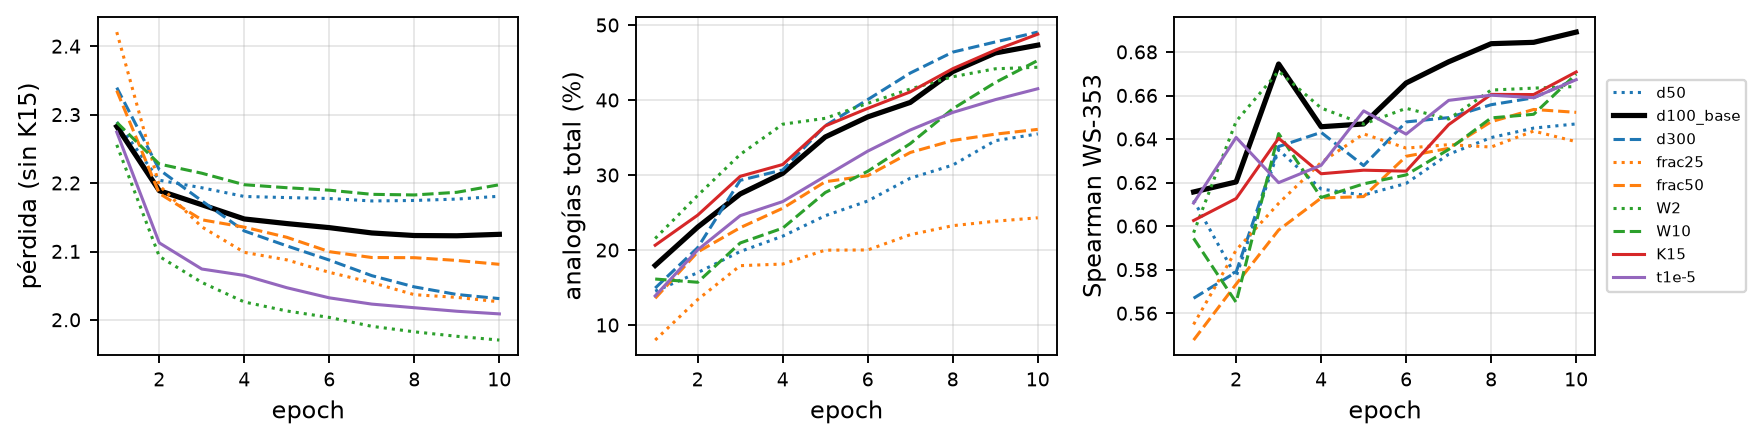
\includegraphics[width=\textwidth]{curvas_compacto.png}
\caption{Pérdida, accuracy de analogías y Spearman WS-353 por epoch para las 9 iteraciones.}\label{fig:curvas}
\end{figure}
Vecinos de control del modelo base (epoch 10): \textit{king}: prince, edward, monarch, throne, queen; \textit{france}: spain, italy, belgium, portugal, netherlands; \textit{computer}: computers, software, simulation, graphics, systems; \textit{good}: bad, excellent, pretty, luck, happy; \textit{january}: february, december, march, november, june; \textit{run}: running, runs, ran, drive, eighth-inning (en el notebook se listan todos los epochs).
\textbf{¿Una pérdida más baja implica mejores embeddings? No.} En la corrida base la pérdida se estanca desde el epoch 8 (2.123$\to$2.125) mientras las analogías suben de 43.8 a 47.3\,\%; entre las corridas con $K{=}5$ la correlación de Spearman entre pérdida final y analogías es 0.12 ($p{=}0.78$): \texttt{frac25} tiene menor pérdida (2.027) que la base (2.125) y solo 24.3\,\% de analogías (vs.\ 47.3\,\%). La pérdida mide la tarea sustituta (distinguir contexto real de ruido), no la geometría del espacio, y no es comparable entre ventanas, submuestreos o $K$ distintos.

\section{Verificación de la aritmética vectorial}
Comparamos el mejor SGNS, el Word2Vec de gensim (mismo corpus, vocabulario y configuración; 2.9\,min en CPU de 8 hilos) y GloVe-100. Nuestra \texttt{analogy(a,b,c,k)} usa 3CosAdd sobre vectores normalizados, excluyendo $a,b,c$; coincide con \texttt{most\_similar} de gensim en el \textbf{100\,\%} de 200 preguntas (top-1 y top-5; diferencia máxima de similitud $2.4{\cdot}10^{-7}$).
\textbf{Analogías propias} (27 en 7 tipos; top-1 / top-5 en \%): género 80/80 en los tres modelos; país--capital 25/75 (SGNS), 25/50 (gensim), 100/100 (GloVe); país--gentilicio 100/100 en los tres; comparativos 75/100 en los tres; superlativos 33/67, 33/33, 67/67; tiempos verbales 100/100, 100/100, 75/100; plurales 100/100, 100/100, 75/100. \textbf{Total:} SGNS 74/89, gensim 74/81, GloVe 81/93; coseno medio de la respuesta correcta con el vector resultante 0.69, 0.70 y 0.83. La tabla completa con top-5, similitudes y rangos está en el notebook (secc.~5.1). \textbf{Sin excluir la consulta}, el primer lugar es $c$ en el 48\,\% (SGNS), 44\,\% (gensim) y 33\,\% (GloVe) de los casos, $b$ en 26/22/11\,\%, y la respuesta correcta solo en 22/30/48\,\%; en \texttt{man:woman::king} los tres devuelven \textit{king} (0.77/0.77/0.84) antes que \textit{queen} (0.72/0.70/0.77).

\textbf{Benchmark por categoría} (vocabulario compartido: las 30\,000 palabras más frecuentes presentes en los tres modelos, ordenadas por frecuencia en nuestro corpus; \textbf{11\,611 de 19\,544 preguntas, 59.4\,\%}, idénticas para los tres):
\begin{table}[H]\centering\scriptsize
\resizebox{0.86\textwidth}{!}{\begin{tabular}{lrrrrrr}
\toprule
Categoría & SGNS add & SGNS mul & gensim add & gensim mul & GloVe add & GloVe mul \\
\midrule
capital common countries & 71.3 & 66.6 & 57.1 & 53.4 & 92.9 & 91.1 \\
capital world & 55.2 & 47.6 & 43.0 & 38.1 & 88.3 & 85.9 \\
currency & 0.0 & 1.4 & 0.0 & 1.4 & 5.7 & 5.7 \\
city in state & 29.5 & 24.8 & 27.0 & 25.1 & 30.9 & 27.8 \\
family & 48.0 & 45.0 & 52.3 & 48.8 & 88.0 & 86.8 \\
g1 adjective to adverb & 15.4 & 11.1 & 16.6 & 13.2 & 27.8 & 27.8 \\
g2 opposite & 9.2 & 7.0 & 11.8 & 8.5 & 27.2 & 23.9 \\
g3 comparative & 48.9 & 45.3 & 56.8 & 54.9 & 80.3 & 78.2 \\
g4 superlative & 30.8 & 31.1 & 30.8 & 31.2 & 61.4 & 62.1 \\
g5 present participle & 40.3 & 32.0 & 42.9 & 39.2 & 72.2 & 71.7 \\
g6 nationality adjective & 83.7 & 81.8 & 81.0 & 78.7 & 97.4 & 95.8 \\
g7 past tense & 66.0 & 58.9 & 62.2 & 57.0 & 58.8 & 56.2 \\
g8 plural & 50.6 & 42.7 & 42.8 & 35.3 & 79.9 & 76.2 \\
g9 plural verbs & 32.9 & 32.6 & 36.3 & 35.4 & 58.3 & 60.9 \\
semántica & 43.3 & 38.0 & 37.3 & 34.1 & 60.6 & 58.1 \\
sintáctica & 49.0 & 44.7 & 49.1 & 45.9 & 68.3 & 67.0 \\
TOTAL & 47.3 & 42.7 & 45.6 & 42.4 & 66.0 & 64.4 \\
\bottomrule
\end{tabular}}
\caption{Accuracy (\%) por categoría de \texttt{questions-words.txt} con 3CosAdd (\textit{add}) y 3CosMul (\textit{mul}).}\label{tab:cat}
\end{table}
\textbf{Paralelismo} (coseno medio entre vectores diferencia $\hat b-\hat a$ de pares de una misma categoría): SGNS 0.226, gensim 0.243, GloVe 0.406, frente a $\approx$0.00 en pares aleatorios; la mejor categoría es \textit{nationality-adjective} (0.45/0.48/0.75). \textbf{t-SNE} de 478 palabras en 15 grupos temáticos (notebook, secc.~5.2): los grupos se forman (países, números, meses/días, colores, familia, deportes, comida) con algo de mezcla entre ciudades y países y entre animales y comida; silueta coseno 0.172 (SGNS) vs.\ 0.201 (GloVe).
\begin{figure}[H]\centering
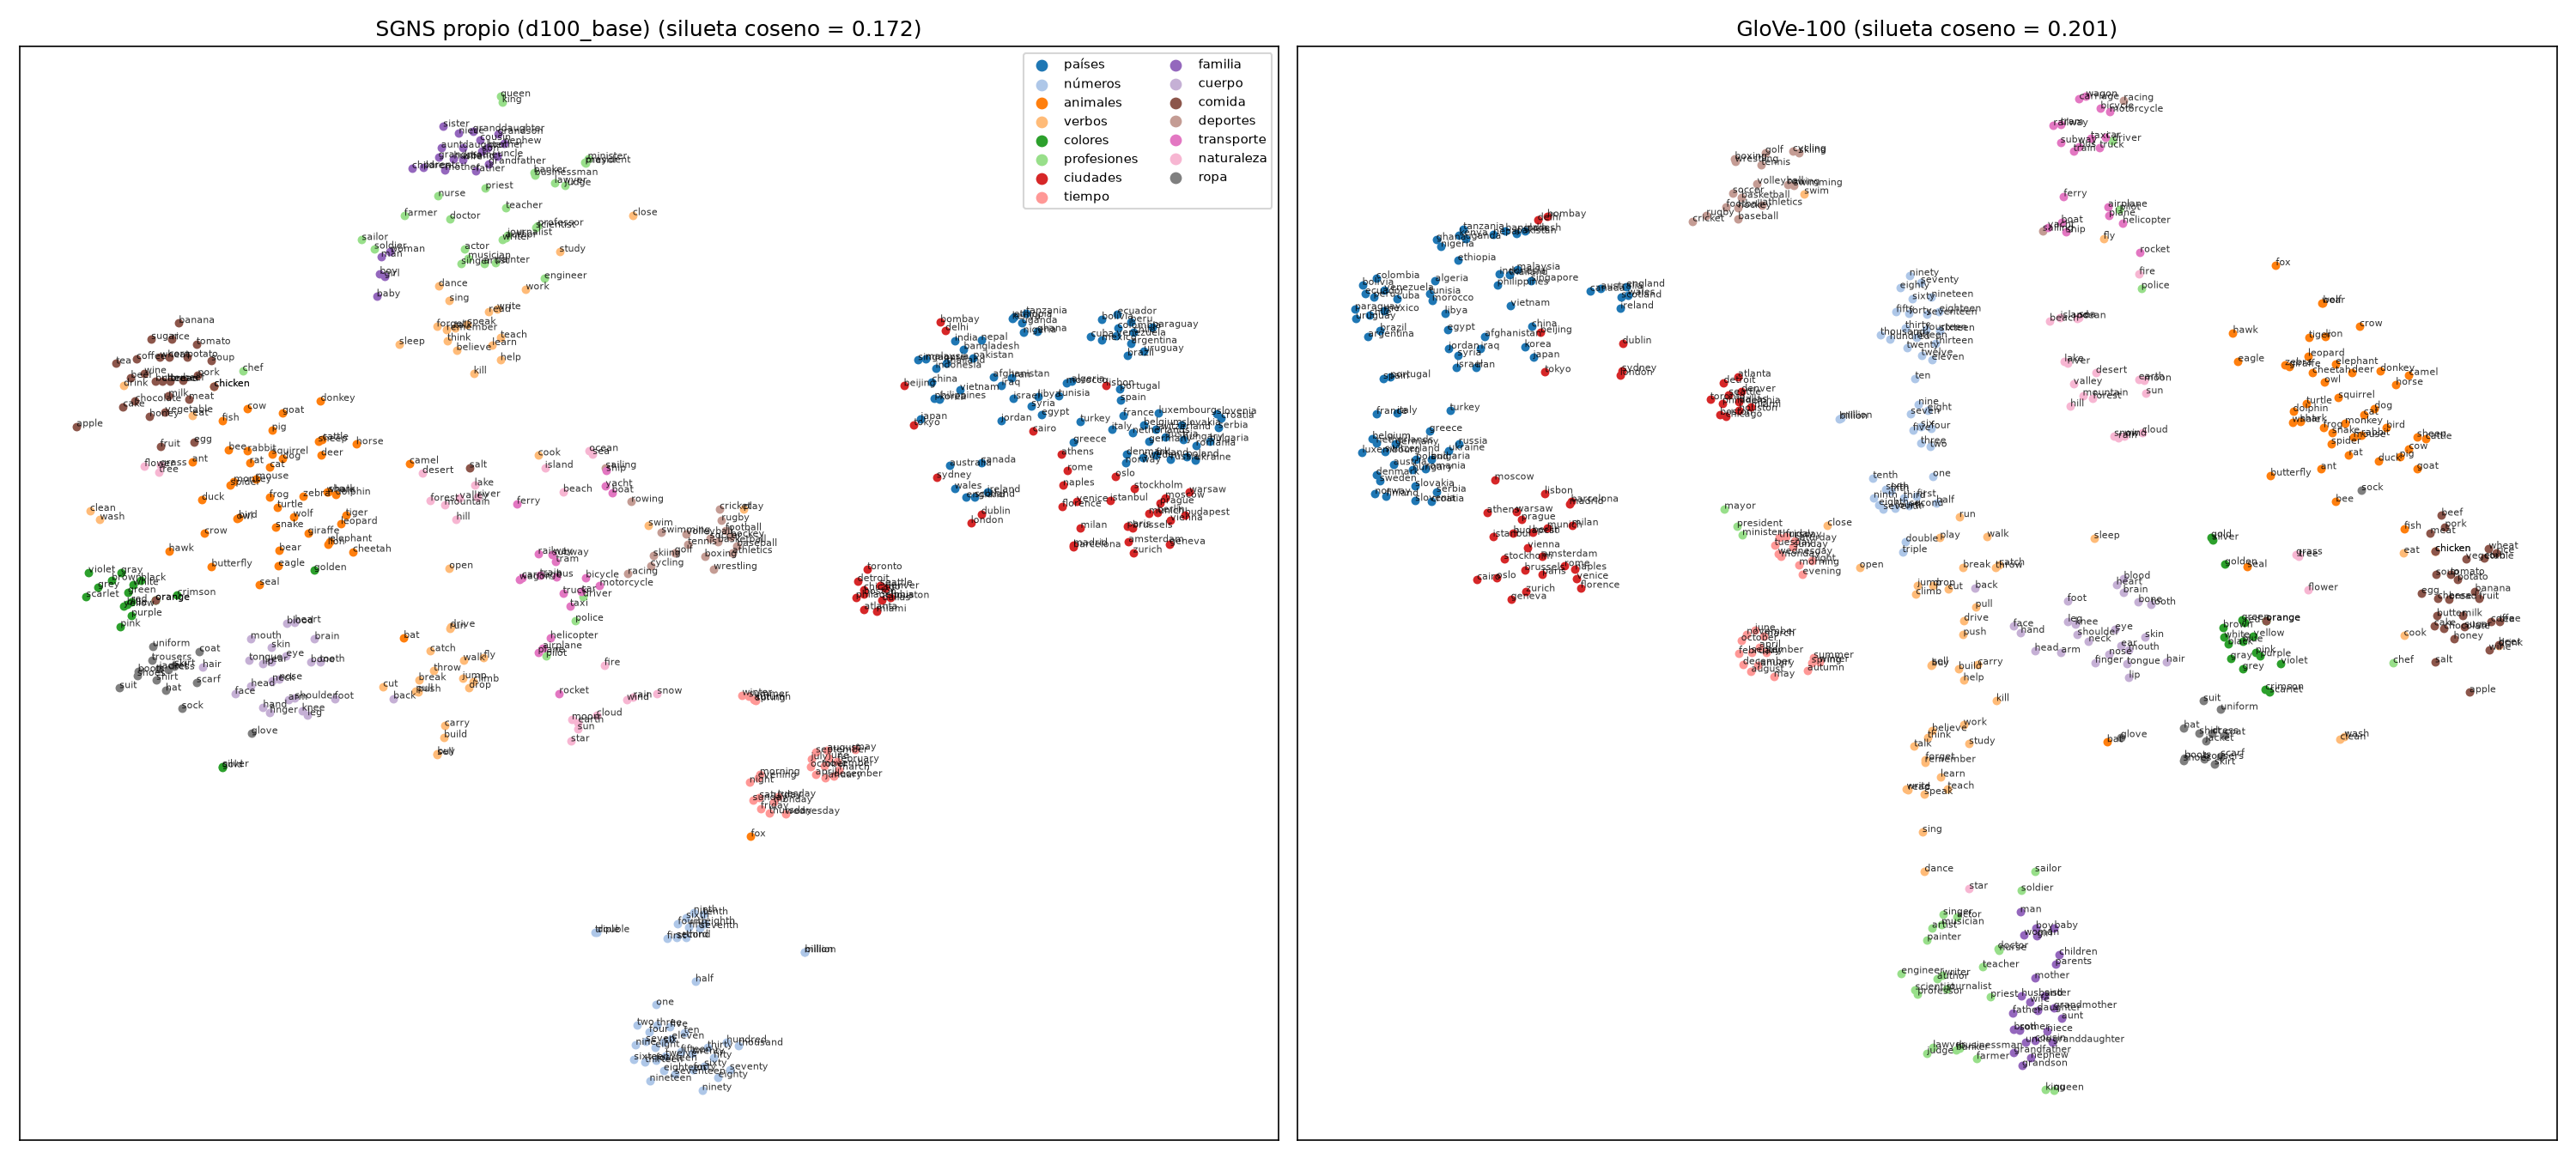
\includegraphics[width=0.93\textwidth]{tsne.png}
\caption{t-SNE (perplejidad 30, distancia coseno) de 478 palabras de 15 grupos temáticos: SGNS propio (izq.) y GloVe-100 (der.).}\label{fig:tsne}
\end{figure}

\section{Clasificación de AG News}
108\,000 / 12\,000 / 7\,600 (train / validación estratificada / test oficial), mismo \texttt{tokenize()}; \texttt{EmbeddingBag(mean)} $\to$ MLP (256) con dropout 0.3, Adam, mejor epoch según F1 de validación (40 epochs en las variantes congeladas, 10 en el resto). Tokens de AG News fuera del vocabulario: \textbf{3.12\,\%} (SGNS y gensim, $|V|{=}100\,844$) y \textbf{0.88\,\%} (GloVe, 400\,000).
\begin{table}[H]\centering\footnotesize
\begin{tabular}{llrrrrrrrr}
\toprule
Modelo & Variante & Params tot. & Entren. & s & Acc val & P val & R val & F1 val & \textbf{F1 test} (Acc) \\
\midrule
TF-IDF + LogReg & $C{=}10$, 1--2-gramas & 1.74\,M & 1.74\,M & 146 & .9295 & .9293 & .9295 & .9294 & \textbf{.9262} (.9263) \\
Aleatorio & entrenado & 4.81\,M & 4.81\,M & 15 & .9130 & .9129 & .9130 & .9129 & .9082 (.9083) \\
SGNS & congelado & 10.11\,M & 26\,884 & 22 & .8978 & .8979 & .8978 & .8976 & -- \\
SGNS & fine-tuning & 10.11\,M & 10.11\,M & 23 & .9189 & .9197 & .9189 & .9188 & .9151 (.9151) \\
gensim & congelado & 10.11\,M & 26\,884 & 22 & .9012 & .9010 & .9012 & .9010 & -- \\
gensim & fine-tuning & 10.11\,M & 10.11\,M & 24 & .9189 & .9197 & .9189 & .9187 & .9139 (.9141) \\
GloVe & congelado & 40.03\,M & 26\,884 & 22 & .9132 & .9134 & .9132 & .9131 & -- \\
GloVe & fine-tuning & 40.03\,M & 40.03\,M & 72 & .9248 & .9253 & .9248 & .9247 & .9213 (.9213) \\
\bottomrule
\end{tabular}
\caption{AG News: métricas macro en validación (todas las variantes) y F1 de test de la mejor variante de cada inicialización (evaluada una sola vez).}\label{tab:cls}
\end{table}
\begin{figure}[H]\centering
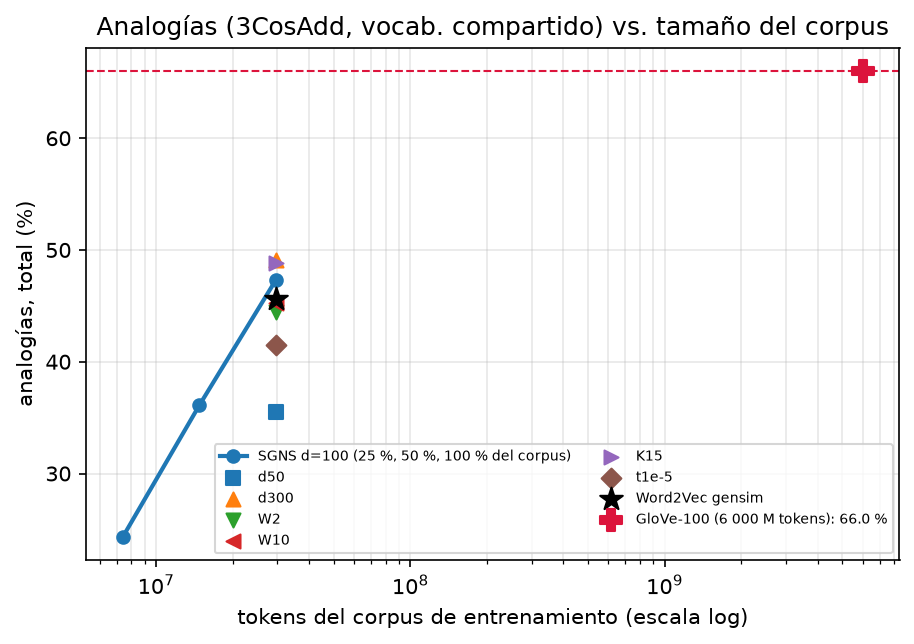
\includegraphics[width=0.49\textwidth]{analogias_vs_tokens.png}\hfill
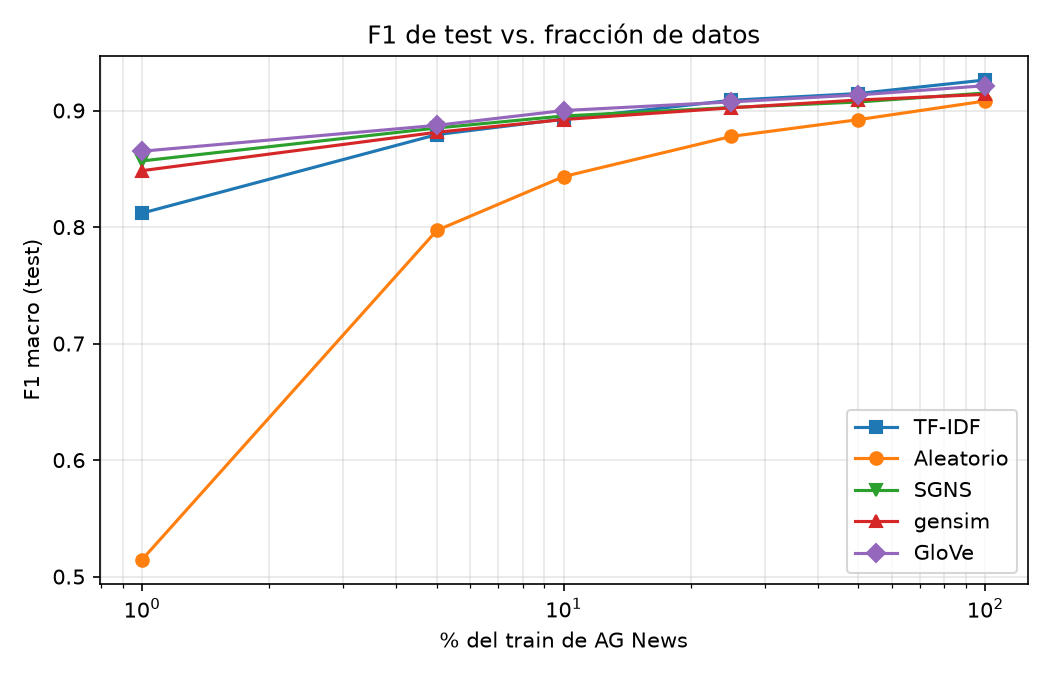
\includegraphics[width=0.49\textwidth]{f1_vs_fraccion.png}
\caption{Izq.: analogías (3CosAdd, vocabulario compartido) vs.\ tokens del corpus para las 9 iteraciones, gensim y GloVe (6\,000\,M de tokens). Der.: F1 de test vs.\ fracción del train de AG News (una curva por inicialización; en cada punto, mejor variante según validación).}\label{fig:two}
\end{figure}
La matriz de confusión de cada modelo está en el notebook (secc.~6.2). SimLex-999 (reservado): SGNS 0.294, gensim 0.316, GloVe 0.298.

\section{Comparación de resultados}
\begin{table}[H]\centering\footnotesize
\resizebox{\textwidth}{!}{\begin{tabular}{p{5.6cm}lll}
\toprule
Métrica & SGNS (propio) & Word2Vec gensim & GloVe-100 \\
\midrule
Tokens del corpus de entrenamiento & 29,604,250 & 29,604,250 & 6 000 000 000 \\
Tamaño del vocabulario & 100,844 & 100,844 & 400,000 \\
Dimensión & 100 & 100 & 100 \\
Tiempo de entrenamiento & 7.6 min (45 s/epoch x 10) & 2.9 min (18 s/epoch x 10) & matriz X $\approx$ 85 min (1 hilo) + 50 iteraciones* \\
Hardware & GPU GTX 1660 SUPER (6 GB) & CPU Ryzen 7 3700X, 8 hilos & 2 x Xeon E5-2658 2.1 GHz, 32 núcleos* \\
Analogías semánticas \% (3CosAdd / 3CosMul) & 43.3 / 38.0 & 37.3 / 34.1 & 60.6 / 58.1 \\
Analogías sintácticas \% (3CosAdd / 3CosMul) & 49.0 / 44.7 & 49.1 / 45.9 & 68.3 / 67.0 \\
Analogías total \% (3CosAdd / 3CosMul) & 47.3 / 42.7 & 45.6 / 42.4 & 66.0 / 64.4 \\
Spearman WordSim-353 & 0.689 & 0.686 & 0.533 \\
Spearman SimLex-999 & 0.294 & 0.316 & 0.298 \\
Coseno medio entre vectores diferencia (paralelismo) & 0.226 & 0.243 & 0.406 \\
Tokens de AG News fuera del vocabulario \% & 3.12 & 3.12 & 0.88 \\
F1-macro en test de AG News (variante) & 0.9151 (fine-tuning) & 0.9139 (fine-tuning) & 0.9213 (fine-tuning) \\
\bottomrule
\end{tabular}}
\caption{SGNS propio vs.\ Word2Vec de gensim vs.\ GloVe. $^*$GloVe: tiempos reportados por Pennington et al.\ (2014) (X$\approx$85\,min con 1 hilo; 14\,min/iteración con 300 dim y 32 núcleos; 50 iteraciones para $d<300$); el tiempo por iteración a 100 dim no se reporta.}\label{tab:cmp}
\end{table}

\section{Discusión y conclusiones}
\textbf{Aritmética vectorial.} Se cumple de forma \textit{aproximada y desigual}: SGNS acierta 47.3\,\% del benchmark (GloVe 66.0\,\%), con éxito alto en relaciones frecuentes y regulares (nacionalidad 83.7\,\%, capitales comunes 71.3\,\%, pasado 66.0\,\%) y fallas en \textit{currency} (0\,\%, solo 70 preguntas cubiertas), \textit{opposite} (9.2\,\%), adjetivo$\to$adverbio (15.4\,\%) y \textit{city-in-state} (29.5\,\%). Las sintácticas superan a las semánticas (49.0 vs.\ 43.3\,\%; GloVe 68.3 vs.\ 60.6\,\%), aunque el grupo semántico incluye las categorías más difíciles. \par\smallskip\textbf{¿Es ``$\approx$'' una igualdad? No:} sin excluir la consulta, el vector resultante cae sobre $c$ o $b$ en $\sim$74\,\% de los casos del SGNS; la respuesta correcta tiene coseno medio $\approx$0.69 (no 1) y los vectores diferencia de una misma relación solo comparten dirección parcialmente (coseno 0.23--0.41, frente a 1 si fuese igualdad exacta). \par\smallskip\textbf{Brecha con GloVe} ($-18.7$ puntos en analogías, pero WordSim-353 0.689 vs.\ 0.533 y SimLex empatado): GloVe usó $\approx$203$\times$ más tokens y otro dominio. El Word2Vec de gensim con nuestro corpus obtiene lo mismo que nuestro SGNS (45.6\,\%), por lo que la diferencia no es de implementación; el experimento de corpus (25/50/100\,\%: 24.3/36.1/47.3\,\%, $\approx$+11.5 puntos por duplicación sin saturar; WikiText completo daría $\approx$+20 puntos por extrapolación lineal, que sobreestima) indica que \textit{la mayor parte} de la brecha es tamaño de corpus, aunque no podemos aislar el efecto del método porque no entrenamos GloVe sobre nuestro corpus.
\par\smallskip\textbf{SGNS vs.\ gensim:} comportamiento similar (analogías 47.3 vs.\ 45.6\,\%, WS-353 0.689 vs.\ 0.686); la diferencia semántica (43.3 vs.\ 37.3\,\%) puede deberse al optimizador (SparseAdam con batch 16\,384 vs.\ SGD por par), a la inicialización y a un sesgo de selección (configuración elegida entre 9 corridas con la misma métrica; una sola semilla). \par\smallskip\textbf{Hiperparámetros:} $d$: 50/100/300 $\Rightarrow$ 35.5/47.3/49.1\,\% (d=300 gana en semántica, 56.7\,\%, y pierde en sintaxis y similitud; 2.4$\times$ más tiempo); ventana: las pequeñas favorecen la sintaxis (brecha sintáctica$-$semántica 10.8, 5.7 y 3.1 puntos para $W{=}2,5,10$) y las grandes la semántica ($W{=}10$ cuesta 1.8$\times$); $K{=}15$ mejora las analogías (48.8\,\%) pero empeora WordSim (0.671) y cuesta 1.7$\times$; $t{=}10^{-5}$ descarta demasiado (41.5\,\%). \par\smallskip\textbf{AG News:} con todos los datos, TF-IDF (.926) $\ge$ GloVe (.921) $>$ SGNS (.915) $\approx$ gensim (.914) $>$ aleatorio (.908): los preentrenados superan a los aleatorios (+1.3 y +0.7 puntos) pero no a TF-IDF con bigramas, que conserva información de orden que el promedio pierde (la diferencia de 0.5 puntos es del orden del error estándar, $\approx$0.3). Con \textbf{1\,\%} de los datos (1\,080 noticias) la ventaja es clara: GloVe .865, SGNS .857, gensim .848, TF-IDF .812, aleatorio \textbf{.515}; TF-IDF empata o gana desde $\approx$25\,\%. \textbf{Congelar} convino con el 1\,\% (GloVe .872 vs.\ .854 en validación con fine-tuning, que sobreajusta); desde el 5\,\% el \textbf{fine-tuning} gana (+1.2 puntos en GloVe y +2.1 en SGNS con el 100\,\%). \par\smallskip\textbf{Limitaciones:} una semilla, subconjunto de 29.6\,M de los 97.5\,M de tokens, búsqueda de hiperparámetros de una variable a la vez.

\vspace{3pt}\textbf{Repositorio:} \repourl
\end{document}
